\chapter{User Interface and Features}
\label{ch:ui}

\section{Wireframes and User Journey}

Wireframes provide a visual outline of the project’s user interface structure and play a key role in mapping the user journey. They enable early visualization of layout and user interactions, offering insight into user navigation within the system well before the detailed design and coding phases.\\
In the \textbf{ft\_transcendence} project, wireframes and key website screenshots illustrate the user journey. The initial screen allows the user to log in using registered credentials or via their 42 Intra account. New users can register by providing a unique username, a valid email address, and a password. Basic input validation is performed during registration.

\begin{figure}[H]
    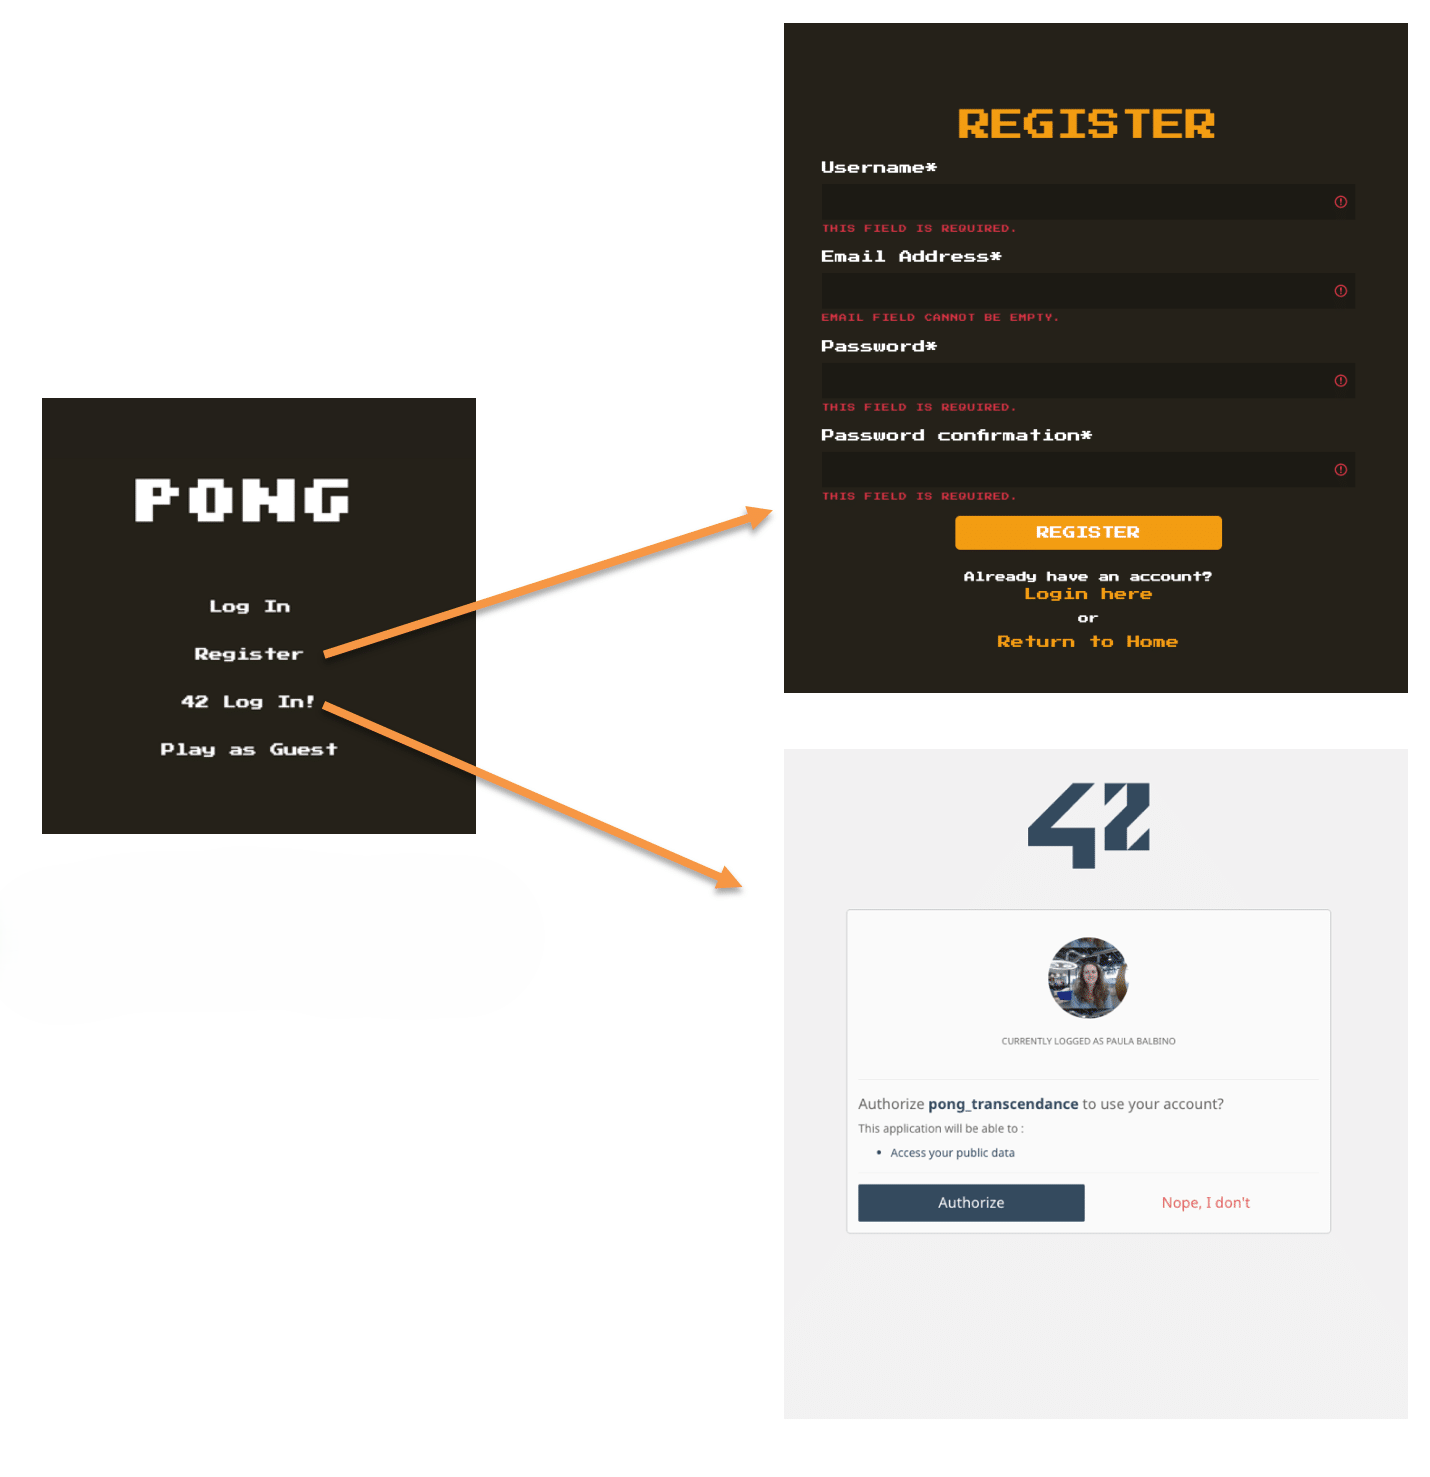
\includegraphics[width=1\linewidth]{images/wireframe-1.png}
    \caption{Initial screen, Login, and Registration options}
    \label{fig:init-screen}
\end{figure}

Once authenticated (either via native login or 42 OAuth), the user is directed to the main dashboard or game selection screen. From here, the user can choose from several Pong game modes: playing a \textbf{1 vs 1} match against another online user, playing against an \textbf{AI opponent}, engaging in a \textbf{4-player local multiplayer} match, or participating in a \textbf{Tournament}. Users can also access their profile and manage friends.

\begin{figure}[H]
    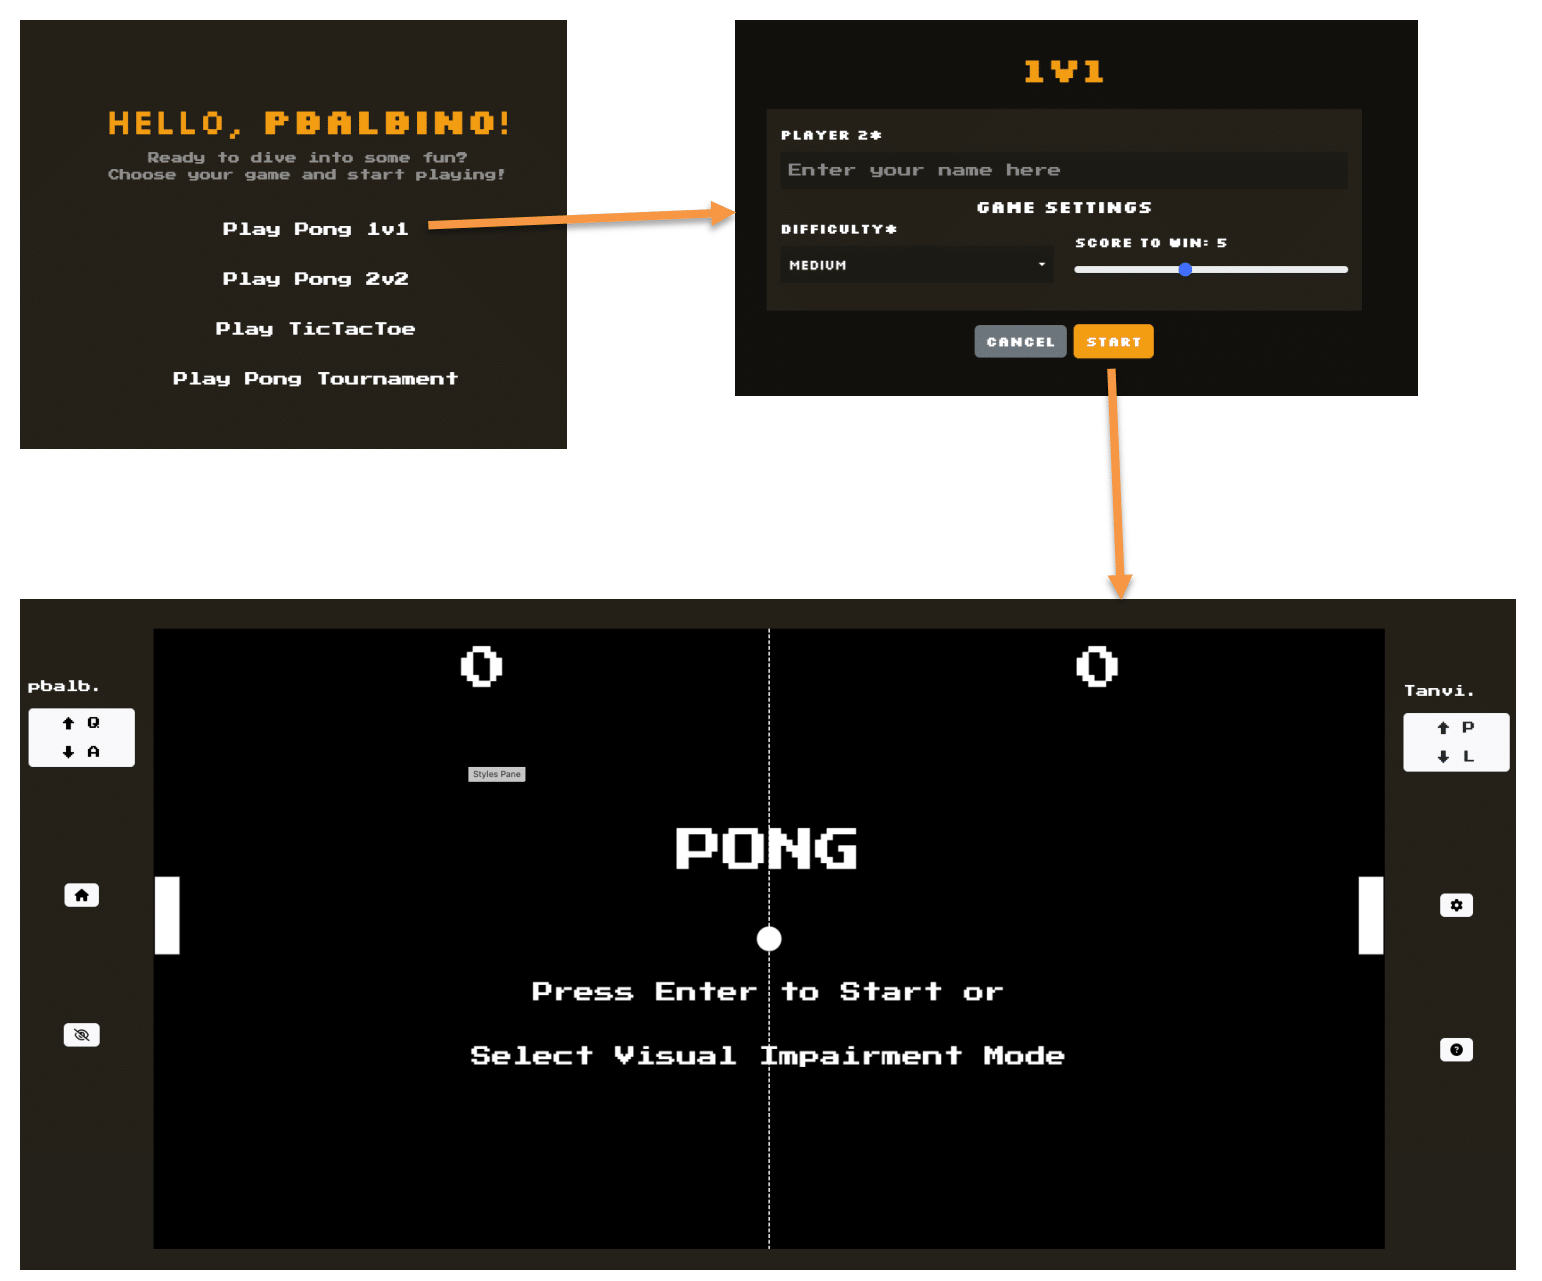
\includegraphics[width=1\linewidth]{images/wireframe-2.png}
    \caption{Game Mode Selection}
    \label{fig:game-selection}
\end{figure}

Selecting a game mode like 1 vs 1 might involve matchmaking or inviting an opponent. Upon starting a match, the Pong game interface is displayed. Player names (or identifiers) are shown, often near indicators for their keyboard controls (e.g., W/S for one player, Up/Down arrows for another). The interface typically includes buttons to return to the main menu ('home'), toggle accessibility options (like a visual impairment mode), access game settings, and view game rules.

\begin{figure}[H]
    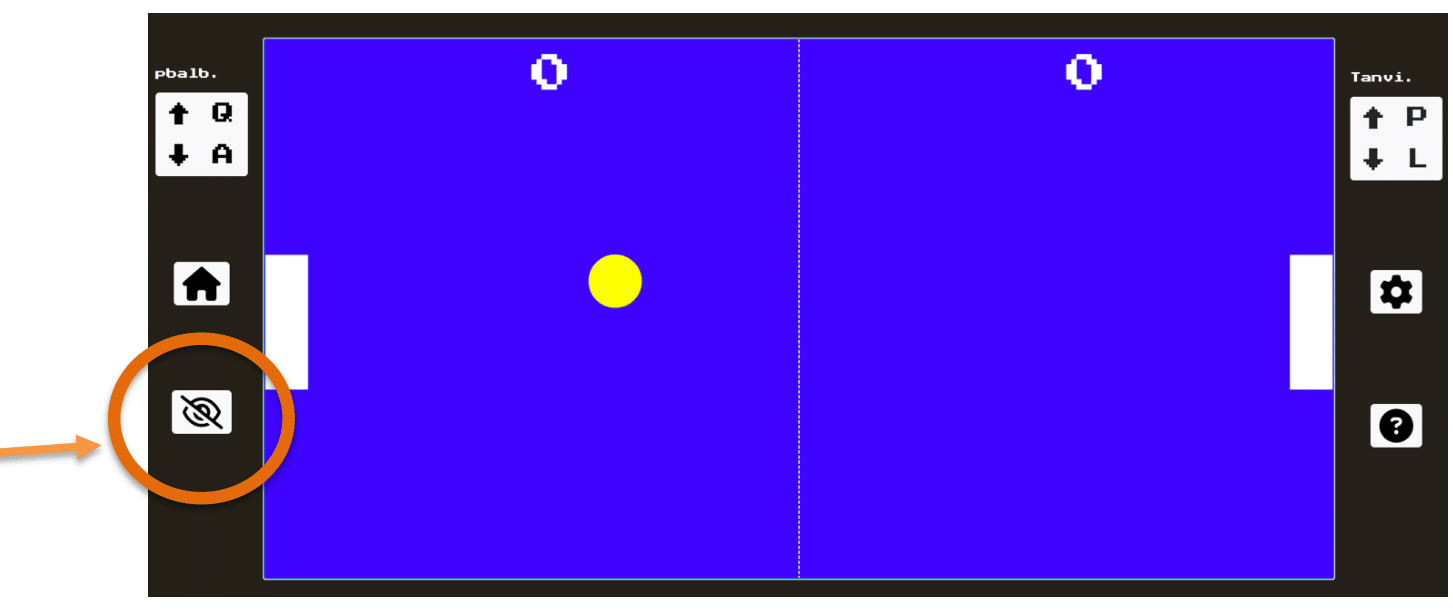
\includegraphics[width=1\linewidth]{images/wireframe-3.png}
    \caption{Pong Gameplay Interface with Accessibility Toggle}
    \label{fig:game-interface}
\end{figure}

If the user activates the visual impairment mode, the display adjusts accordingly, often using high-contrast colors and potentially adapting the appearance of the ball, paddles, and interface elements for better visibility.

\begin{figure}[H]
    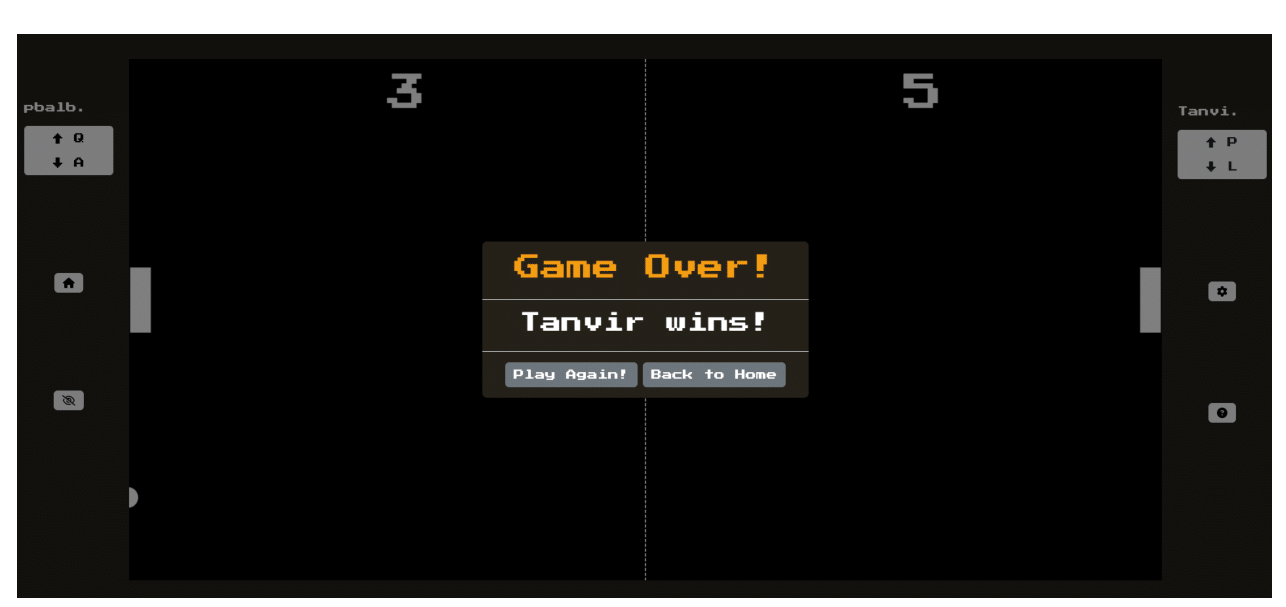
\includegraphics[width=1\linewidth]{images/wireframe-4.png}
    \caption{Visual Impairment Mode Activated}
    \label{fig:impairment-mode}
\end{figure}

When a match concludes (e.g., a player reaches the target score), a game over screen is displayed, indicating the winner. Options are typically presented to return to the main menu or play again (rematch).

\begin{figure}[H]
    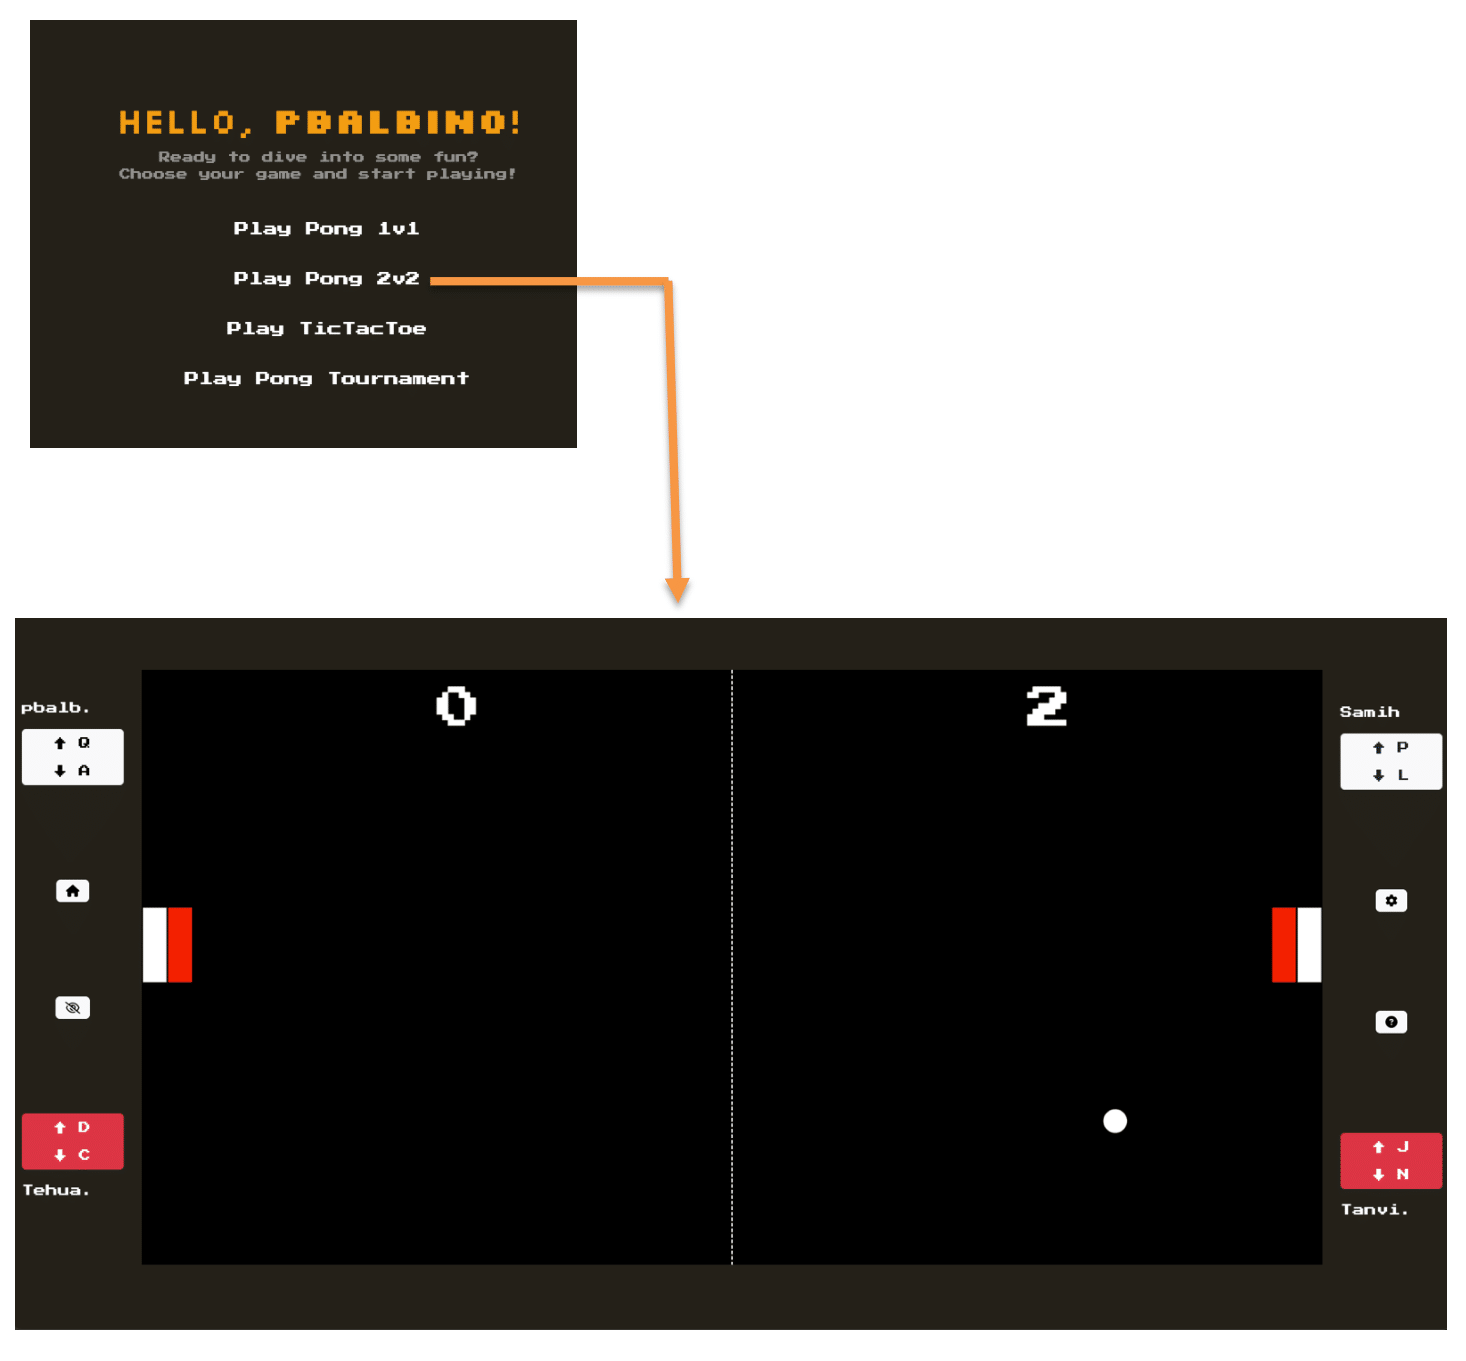
\includegraphics[width=1\linewidth]{images/wireframe-5.png}
    \caption{Pong Match - Game Over Screen}
    \label{fig:gameover}
\end{figure}

The 4-player local mode would adapt the interface to accommodate four paddles and potentially different control schemes.

\begin{figure}[H]
    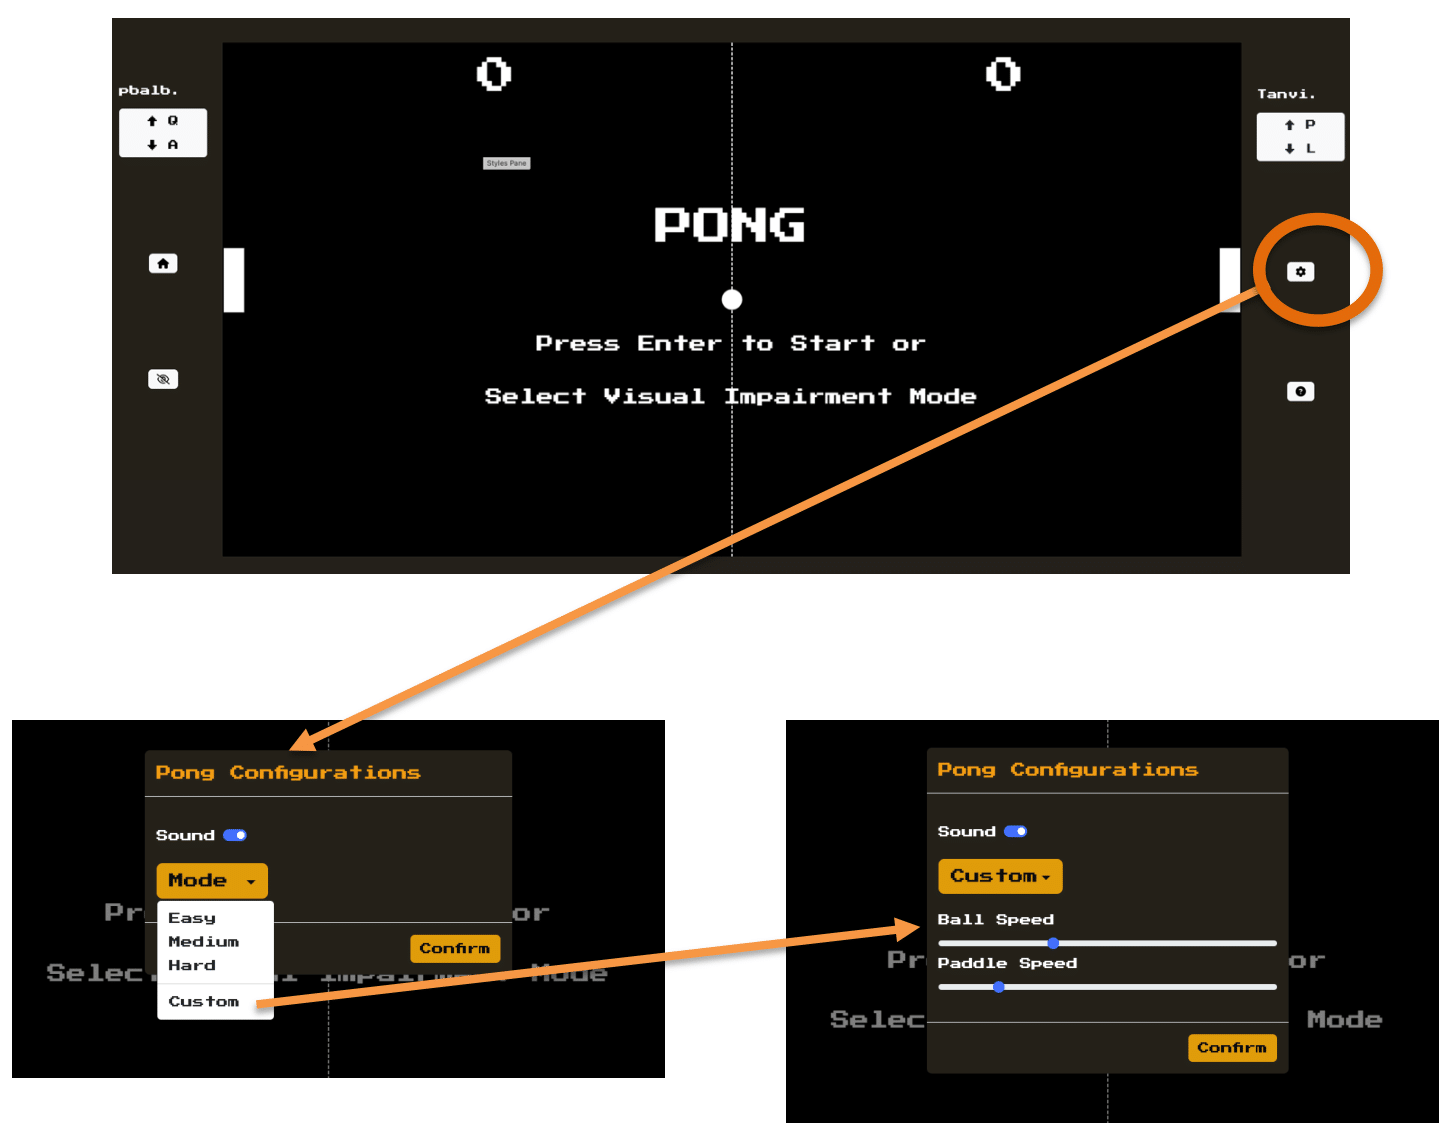
\includegraphics[width=1\linewidth]{images/wireframe-6.png}
    \caption{Illustrative 4-Player Pong Match Layout}
    \label{fig:4player-match}
\end{figure}

Game settings might be accessible via an icon (e.g., a gear). These settings could potentially include options like adjusting AI difficulty (for 'vs AI' mode) or toggling sound effects.

\begin{figure}[H]
    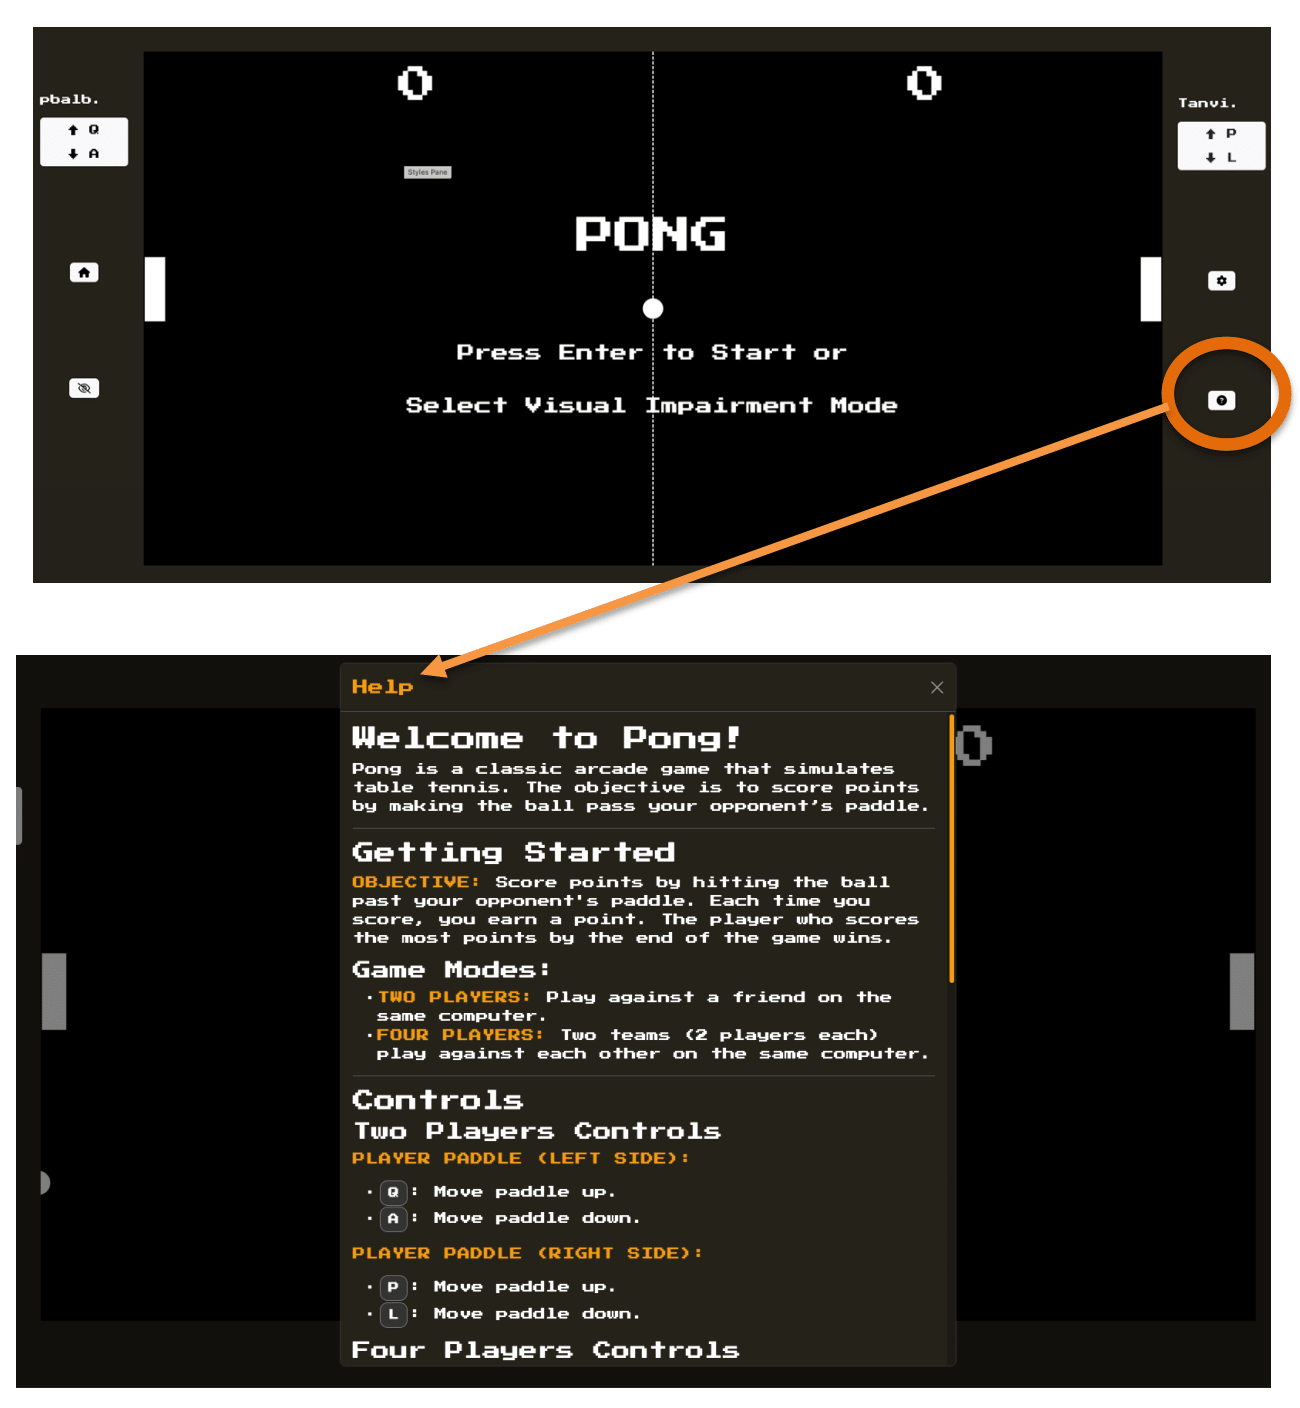
\includegraphics[width=1\linewidth]{images/wireframe-7.png}
    \caption{Potential Pong Game Configuration Options}
    \label{fig:config}
\end{figure}

A help or rules icon might display a popup explaining the basic rules of Pong.

\begin{figure}[H]
    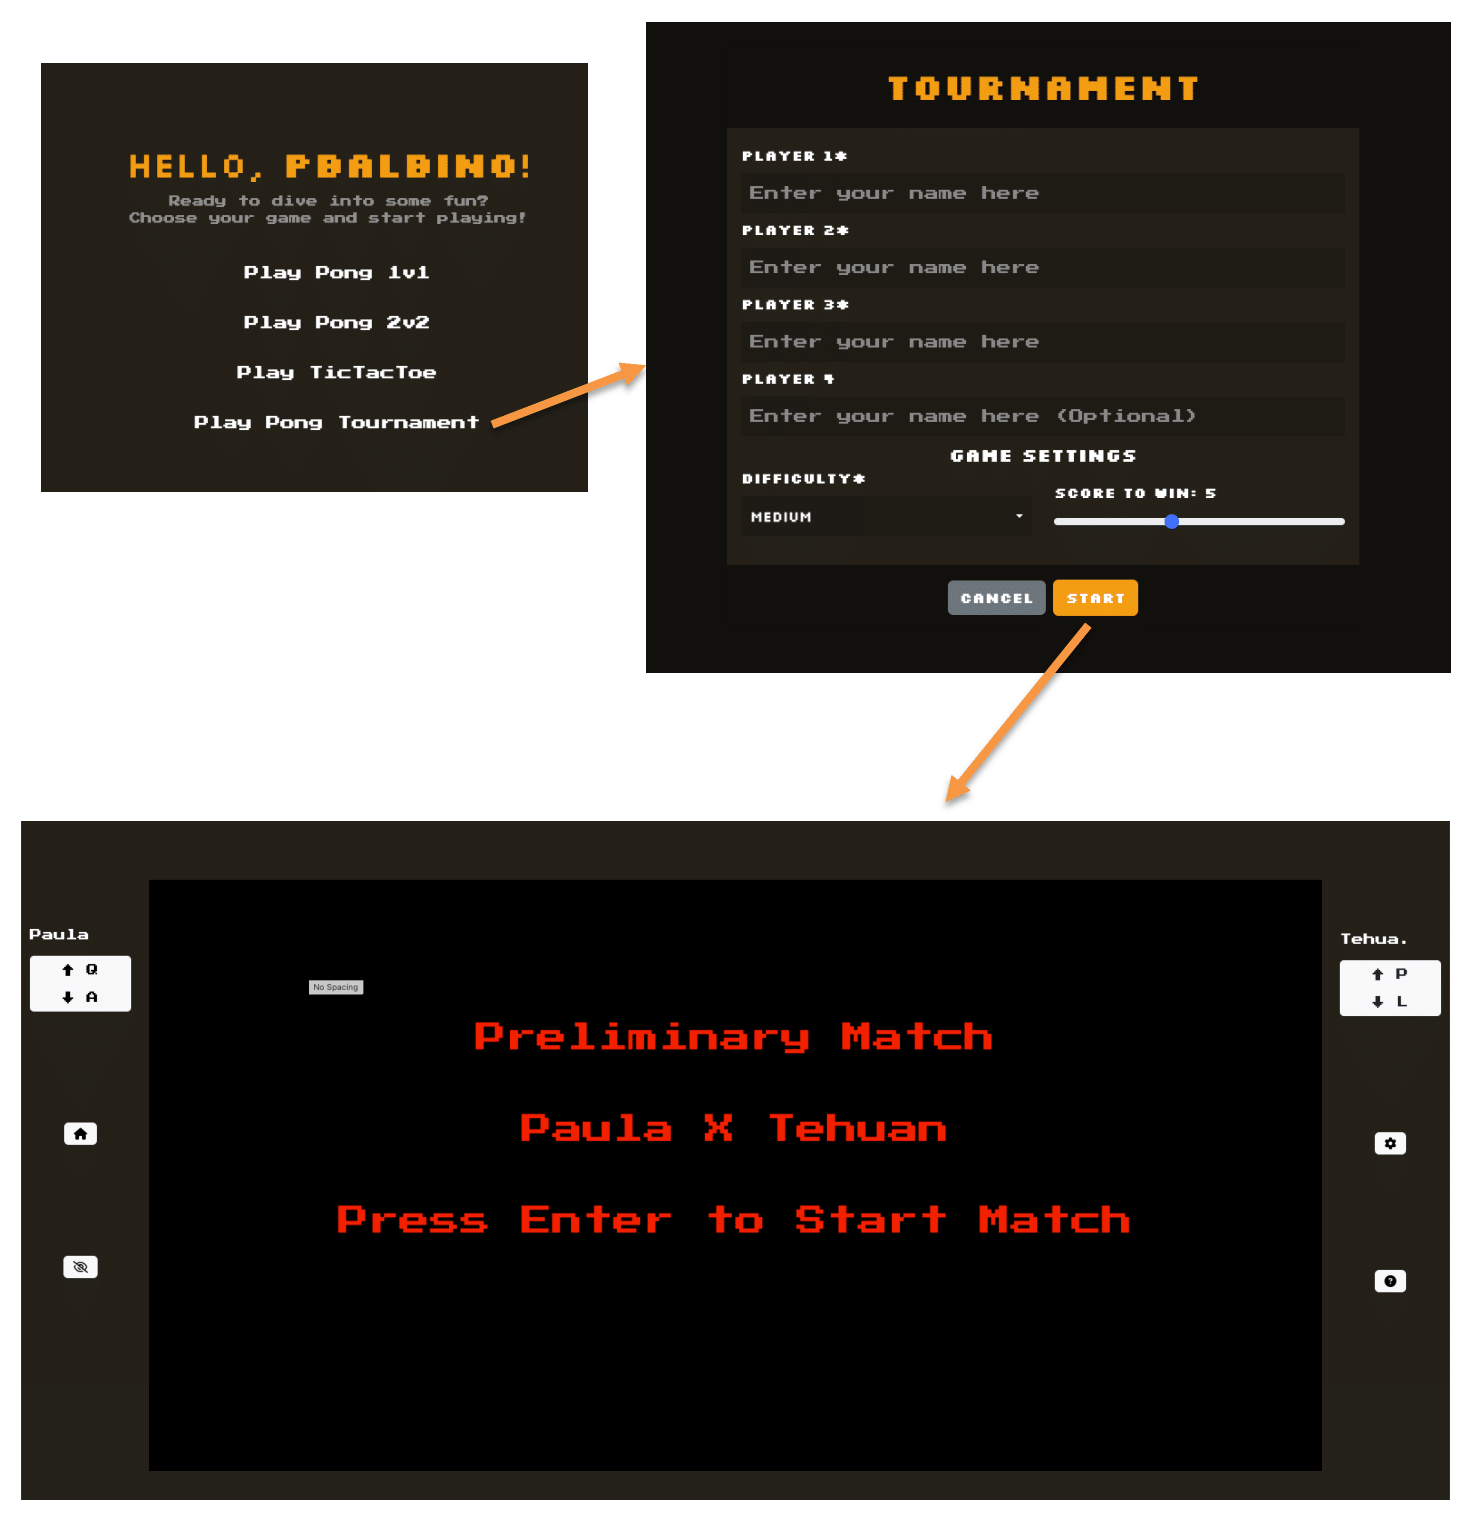
\includegraphics[width=1\linewidth]{images/wireframe-8.png}
    \caption{Pong Game Rules Popup}
    \label{fig:game-rules}
\end{figure}

For \textbf{Tournaments}, the interface would guide users through the bracket. This might involve an initial screen to sign up or view the tournament structure. As matches are played, the bracket view would update to show winners advancing. The final tournament results are recorded in the PostgreSQL database and also immutably on the Ethereum sidechain.

\begin{figure}[H]
    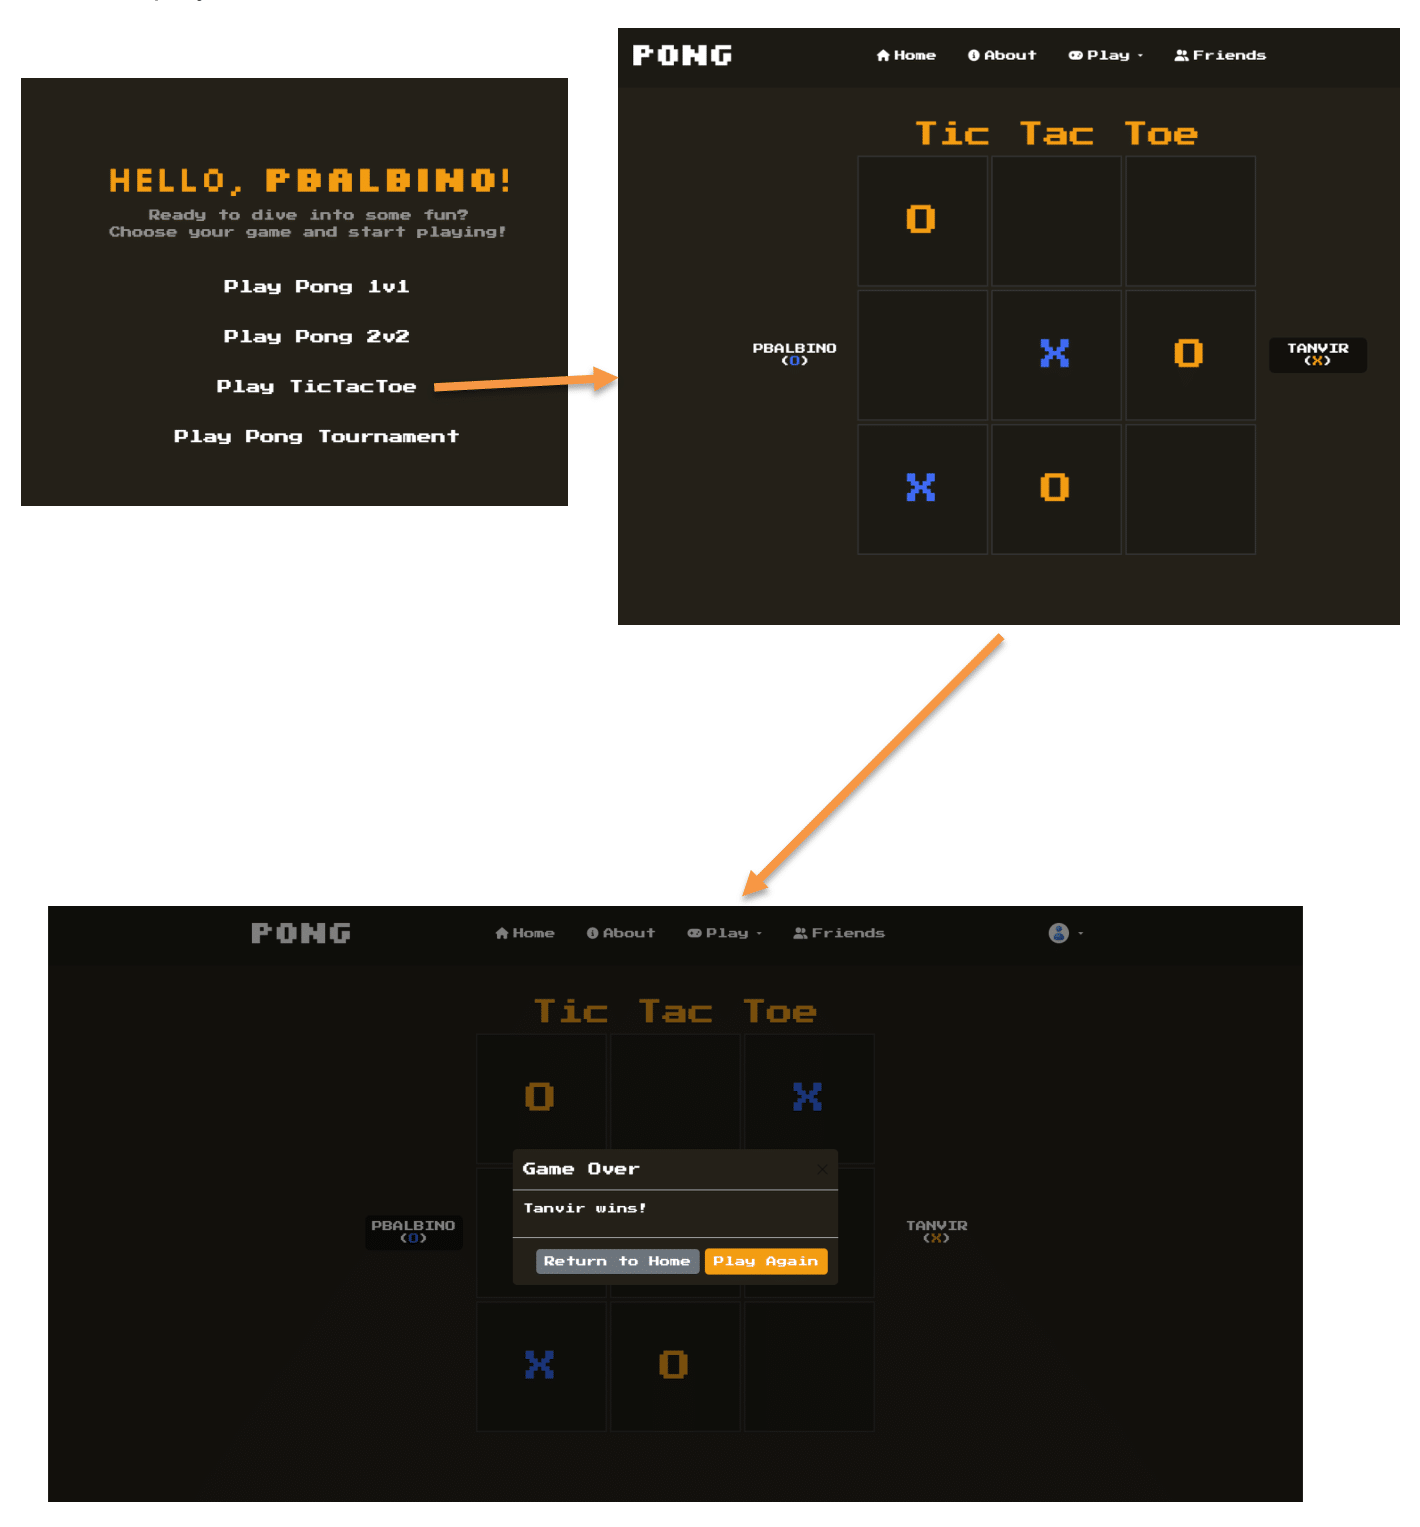
\includegraphics[width=1\linewidth]{images/wireframe-9.png}
    \caption{Illustrative Pong Tournament Bracket View}
    \label{fig:tournament}
\end{figure}

Back on the main dashboard or via a dedicated section, users can manage their \textbf{Friends List}. This involves searching for other users by username and sending friend requests. Appropriate feedback is given if a user does not exist.

\begin{figure}[H]
    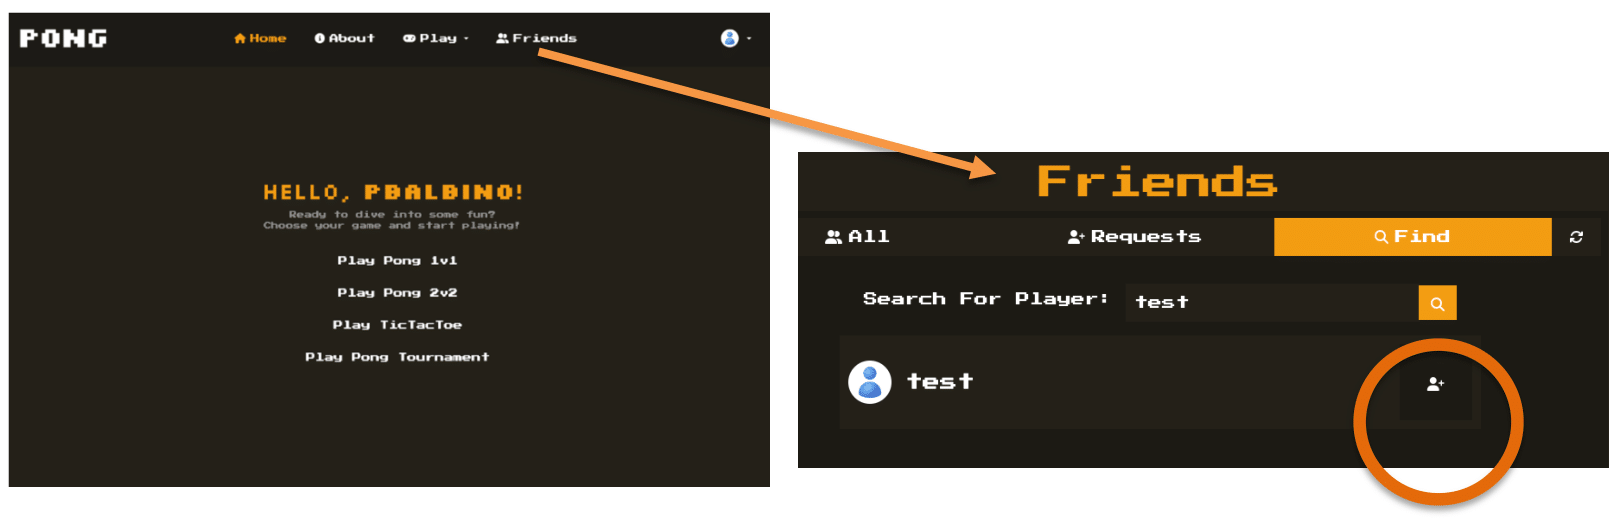
\includegraphics[width=1\linewidth]{images/wireframe-10.png}
    \caption{Friends Page - Adding a Friend}
    \label{fig:friends-add}
\end{figure}

When a user receives a friend request, they are notified (e.g., on their dashboard or friends page) and can choose to accept or reject the request.

\begin{figure}[H]
    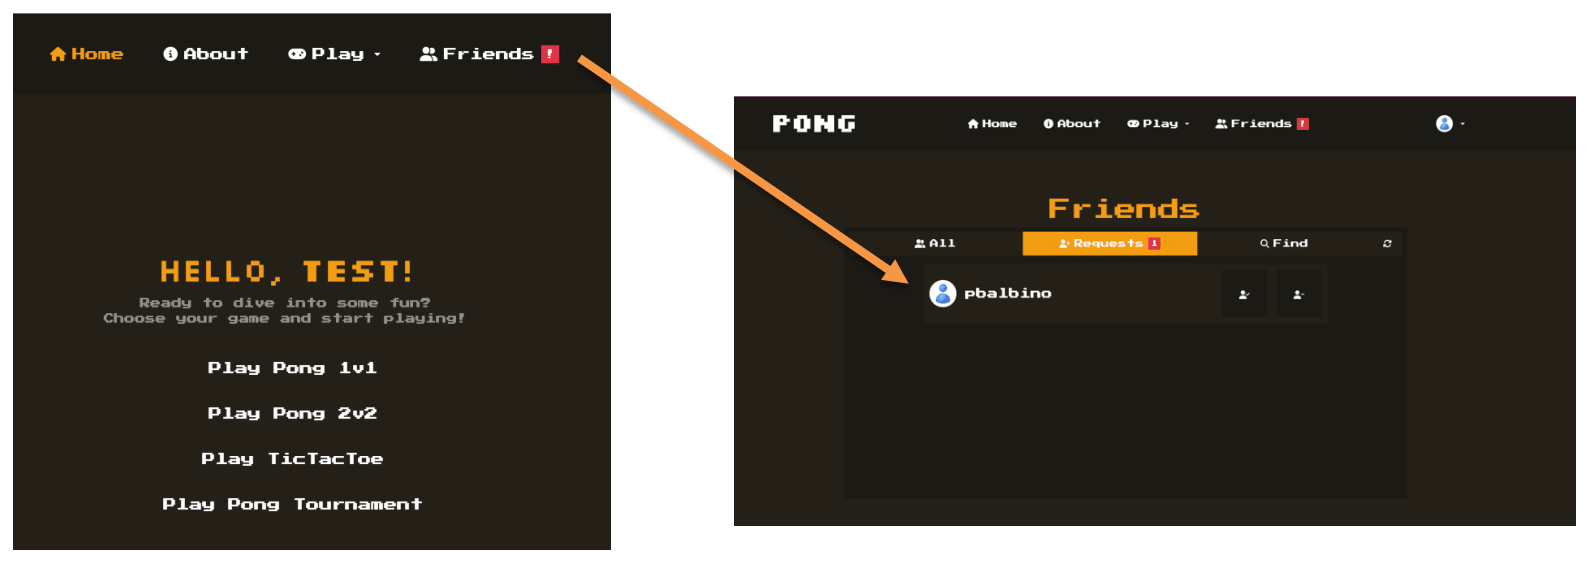
\includegraphics[width=1\linewidth]{images/wireframe-11.png}
    \caption{Friend Request Notification and Approval}
    \label{fig:friends-request}
\end{figure}

Users can access their \textbf{Profile} page, typically via an icon in the header. The profile displays gameplay statistics such as wins and losses, and a history of recent matches played. Users can also edit their profile information, which may include changing their display name or uploading a new avatar.

\begin{figure}[H]
    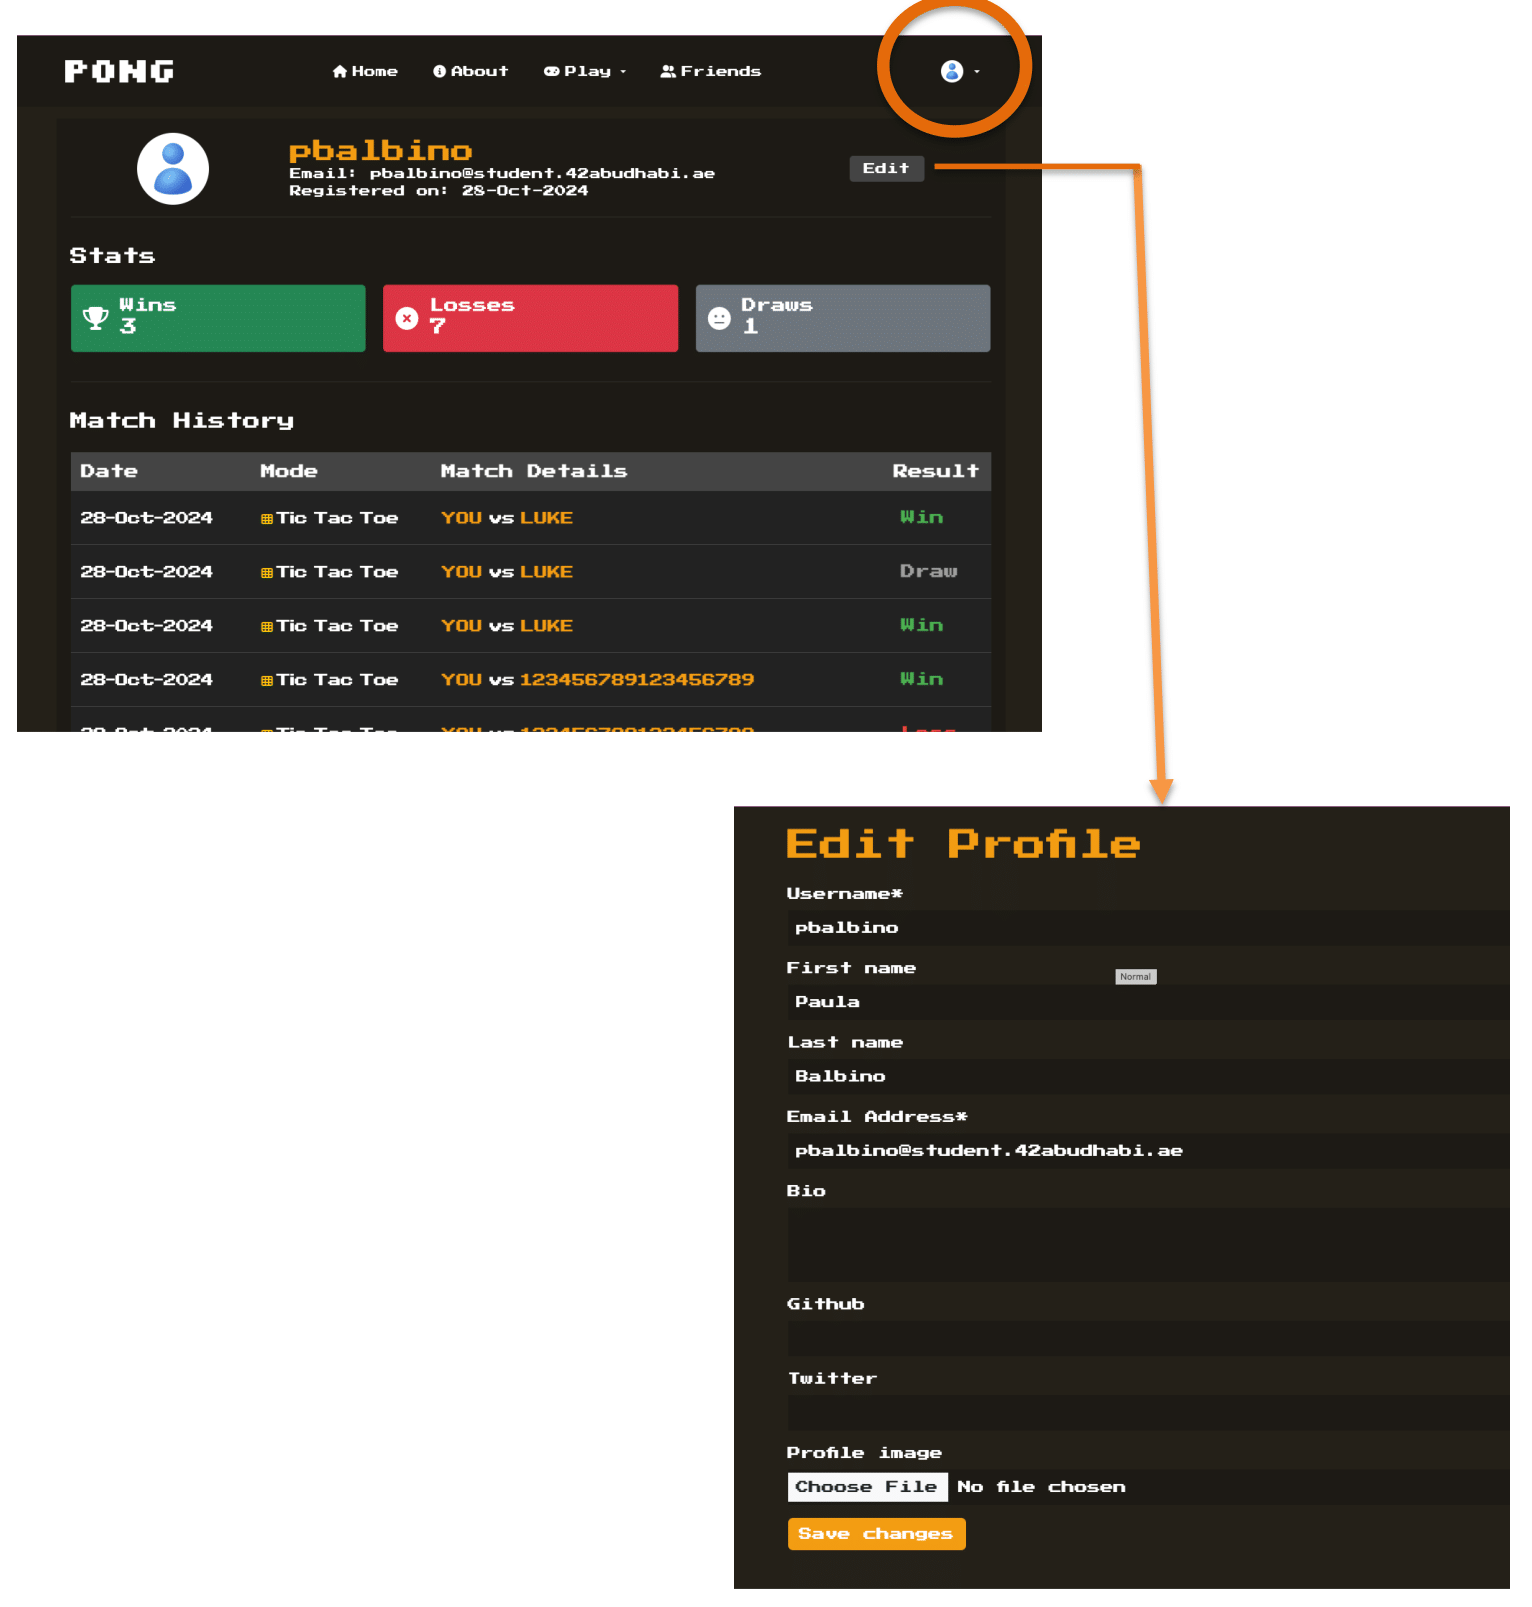
\includegraphics[width=1\linewidth]{images/wireframe-12.png}
    \caption{User Profile Screen with Stats, History, and Edit Option}
    \label{fig:profile-page}
\end{figure}

\textbf{Account Settings} provide options for managing security and account details. Users can enable or disable Two-Factor Authentication (2FA) and change their account password. Setting up 2FA typically involves scanning a QR code with an authenticator app (like Google Authenticator) and verifying a TOTP code.

\begin{figure}[H]
    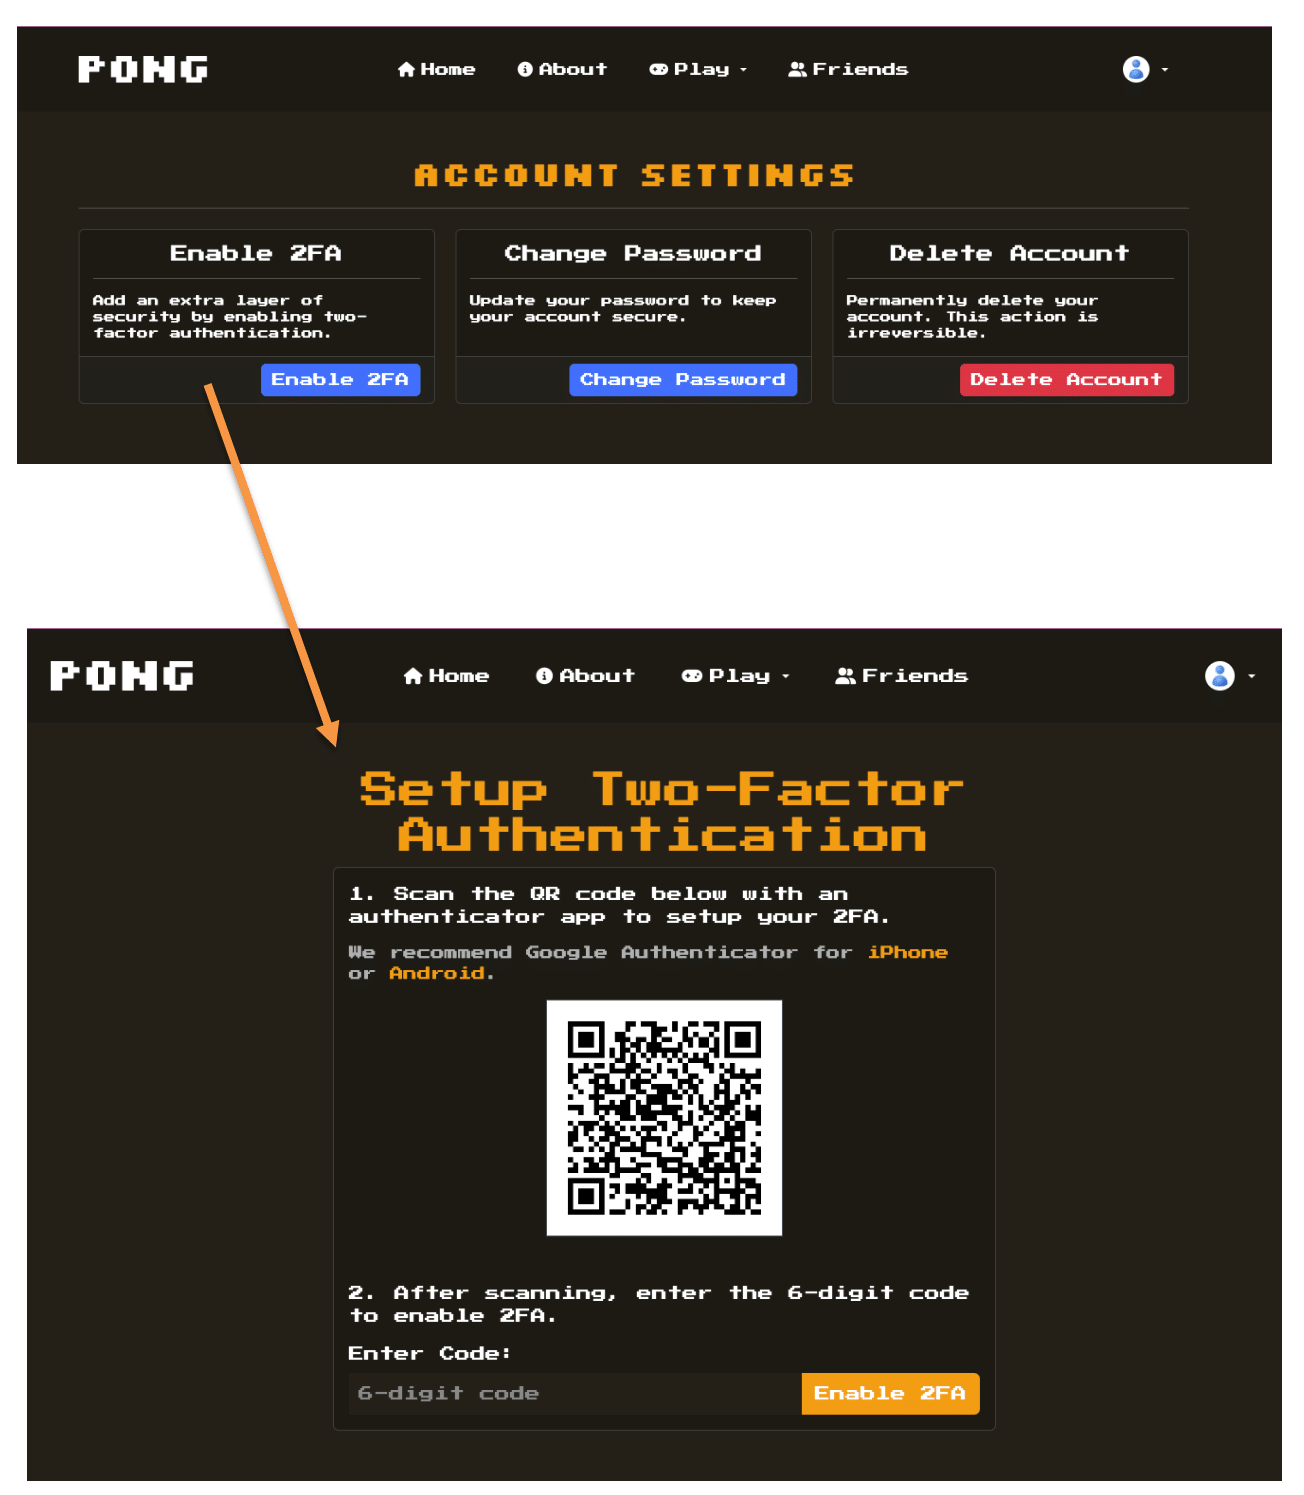
\includegraphics[width=1\linewidth]{images/wireframe-13.png}
    \caption{Account Settings: 2FA Setup and Password Change}
    \label{fig:settings}
\end{figure}

Finally, an \textbf{About} page may provide information about the ft\_transcendence project, the game of Pong, and the development team, potentially including links to their GitHub profiles.

\begin{figure}[H]
    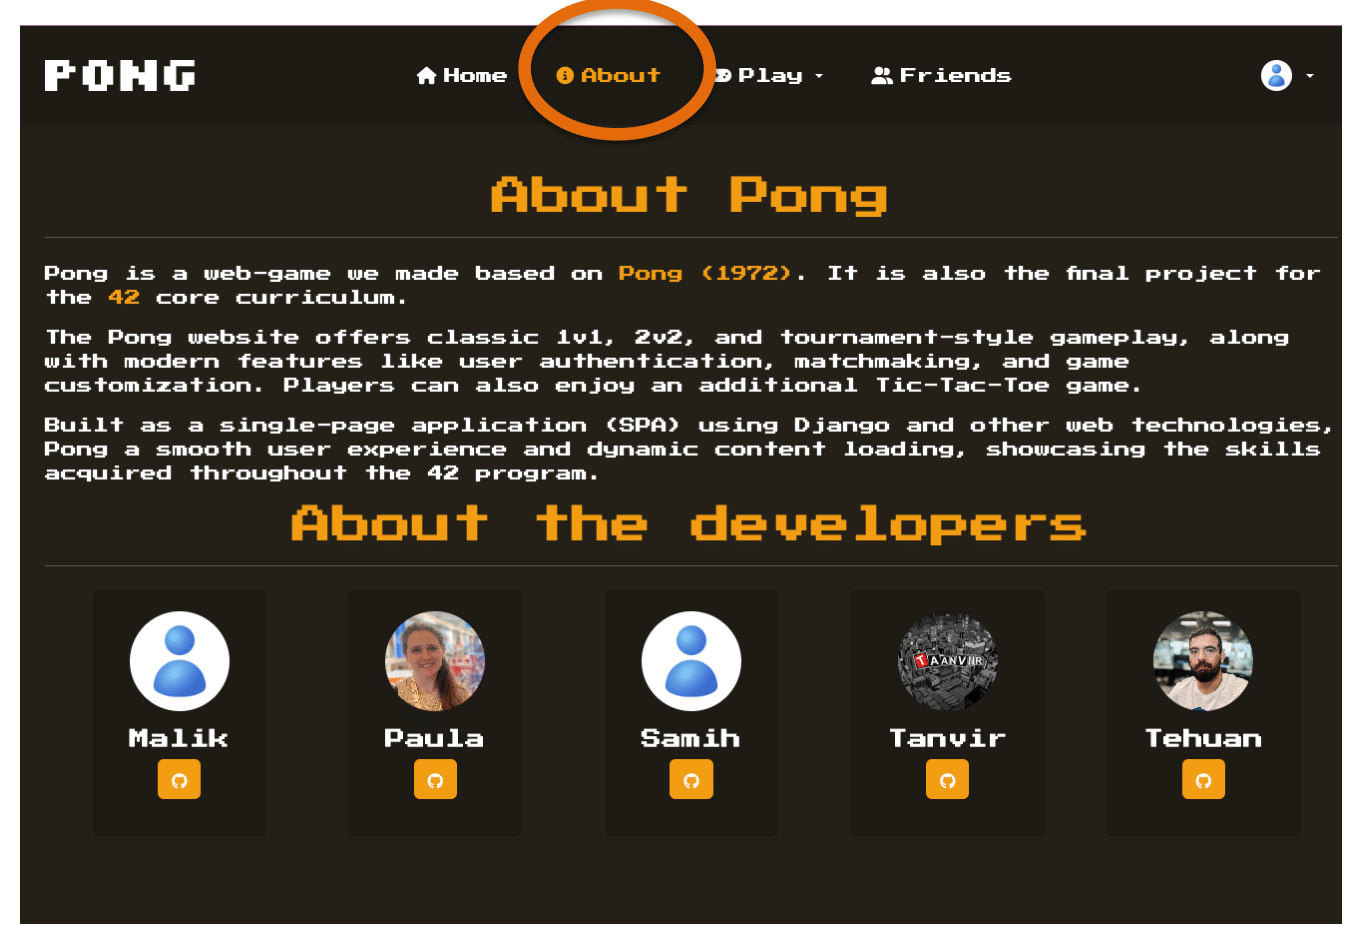
\includegraphics[width=1\linewidth]{images/wireframe-14.png}
    \caption{About Page}
    \label{fig:about-page}
\end{figure}
